77. Приложить друг к другу два прямоугольника можно тремя способами. В первых двух случаях прямоугольники одинаковые, а в третьем --- это прямоугольники $3\times1$ и $9\times3$(он тоже имеет пузатость $3:1$). Получим пузатости $6:1,\ 3:2,\ 10:3.$
\begin{center}
\begin{figure}[ht!]
\center{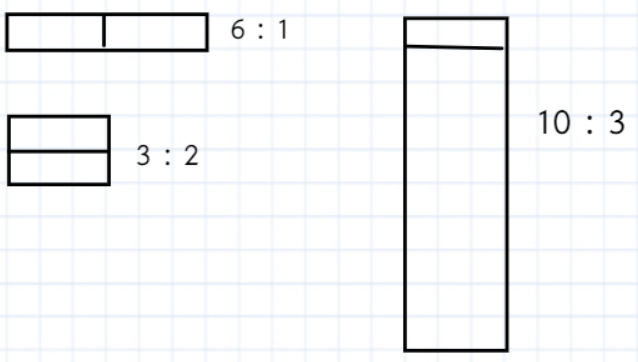
\includegraphics[scale=0.35]{puz.png}}
\end{figure}
\end{center}
